\chapter{Analysis of the Higgs boson at the LHC} \label{chap:chap-4}


% \begin{singlespace}
%     \epigraph{This is a large quote placed with \\ 
%     single spacing over two lines}{-- Unknown Author}
% \end{singlespace}


%% remove the following and add your chapter text here
% \section{A long section heading to test the distance before this}

% \blindtext

% \begin{figure}[ht]
% \begin{center}
%     \includegraphics[width=\textwidth, trim={6cm 5cm 6cm 5cm},clip,page=1] {chap4.pdf}
%     \caption{Here are some photos of ducks to make you feel happy in tough times.}
%     \label{fig:ducks}
% \end{center}
% \end{figure}

% \Blindtext[2]

The standard model (SM) of particle physics postulates the existence of a Higgs field responsible for the
generation of the masses of fundamental particles. The excitation of this
field is known as the Higgs boson ($\PH$)~\cite{StandardModel67_1, Englert:1964et,Higgs:1964ia,
	Higgs:1964pj,Guralnik:1964eu,StandardModel67_2,StandardModel67_3}.
The properties of the \Hboson, observed with a mass of approximately 125\GeV by the ATLAS and CMS
Collaborations~\cite{Aad:2012tfa,Chatrchyan:2012xdj,Chatrchyan:2013lba} at the CERN LHC, are found to be consistent with
the expectations of the SM~\cite{ATLASnature,CMSnature}. The mass of the \Hboson (\mH) is a free parameter of the model and, 
since it determines all other Higgs properties, should be measured with as high precision as possible.
For example, the Higgs boson couplings to vector bosons strongly depend on the \Hboson mass and are precisely predicted by the SM.
Another important \Hboson characteristic is its lifetime, predicted by the SM to be $1.6\times10^{-22}$\,s, corresponding to a total width (\GH) of $4.1$\MeV~\cite{deFlorian:2016spz},
as predicted precisely within the SM for $\mH = 125 \GeV$.
A deviation from the SM prediction would point to either anomalous \Hboson couplings or its decay to yet undiscovered particles.

The ATLAS and CMS Collaborations measured the \Hboson mass to be $125.09 \pm 0.24\GeV$ \cite{Aad:2015zhl} using $\sqrt{s}=7$ and 8\TeV proton-proton ($\Pp\Pp$) collision data from the 2011--2012 data-taking periods (Run 1), corresponding to a total integrated luminosity per experiment of 25\fbinv.
This result has been superseded by both collaborations.
The ATLAS experiment measured the \Hboson mass to be $125.11 \pm 0.11 (\pm 0.09)\GeV$ \cite{ATLAS_mass}, combining the $\PH \to \PGg\PGg$ and \Hfourl ($\Pell = \Pe$, $\PGm$) channels from Run 1 and data collected at $\sqrt{s}=13\TeV$ in 2015--2018 (Run~2).
The value in parentheses is the statistical uncertainty only.
The most recent CMS result, also using the $\PH \to \PGg\PGg$ and \Hfourl channels and including Run 1 and 36\fbinv of $\sqrt{s}=13\TeV$ data from 2016, is 
\mH = $125.38 \pm 0.14$ $(\pm 0.11) \GeV$.
Measurements from ATLAS and CMS using only the \Hfourl channel and 2016 data are $124.94 \pm 0.18 (\pm 0.17)\GeV$ and $125.26 \pm 0.21 (\pm 0.19)\GeV$, respectively.

Considering only on-shell Higgs boson production, CMS set an upper limit 
on the \Hboson width $\GH < 1.10\GeV$ at 95\% confidence level (\CL), 
limited by the four-lepton invariant mass resolution~\cite{Khachatryan:2014jba,Sirunyan:2017exp}.
Both the ATLAS and CMS experiments have also set limits on 
$\GH$~\cite{Khachatryan:2014iha,Aad:2015xua,Khachatryan:2015mma,
	Khachatryan:2016ctc,Aaboud:2018puo,Sirunyan:2019twz,CMS:2022ley}
from an \offshell production method~\cite{Caola:2013yja,Kauer:2012hd,Campbell:2013una},
which relies on the measurement of the ratio of off- to on-shell production rates.
Considering both gluon fusion (\ggH) and electroweak (EW) processes, the most recent measurements are
$\GH= 3.2^{+2.4}_{-1.7}\MeV$ \cite{CMS:2022ley} and $\GH = 4.3^{+3.3}_{-2.5}\MeV$~\cite{atlascollaboration2023evidence} by CMS and ATLAS, respectively.
Finally, from an upper limit on the \Hboson flight distance in the detector,
CMS set a lower limit of $\GH > 3.5\times10^{-9}$\MeV at 95\% \CL~\cite{Khachatryan:2015mma}.

This paper reports an updated CMS measurement of the \Hboson mass and width using \onshell production and the \Hfourl decay.
The data sample includes 138\fbinv of $\Pp\Pp$ collision data at $\sqrt{s}=13\TeV$ collected in 2016--2018, in combination with the Run 1 data.
Compared to the previous CMS \onshell \Hboson measurement in this channel~\cite{Sirunyan:2017exp}, 
the statistical and systematic uncertainties affecting \mH have been reduced by including the beam spot in a refit of the muon tracks; 
adopting an improved event categorization procedure; and performing a detailed study of the lepton momentum scale and resolution.

A measurement of the relative off- and on-shell \Hboson production offers direct information about 
\GH~\cite{Caola:2013yja,Kauer:2012hd,Campbell:2013una}.
For each \Hboson production mechanism $j$, with subsequent decay to four leptons, 
the on- and \offshell cross sections $\sigma_j$ are proportional to
\begin{equation}
	\label{eq:resonant}
	\sigma_j^\text{\onshell} \propto \mu_j^\text{\onshell} 
	\quad\text{and}\quad
	\sigma_j^\text{\offshell} \propto \mu_j^\text{\onshell}  \ \GH,
\end{equation}
where $\mu_j^\text{\onshell}$ is the \onshell signal strength, defined as the ratio of the observed number of \onshell four-lepton events relative to the SM expectation.
The signal strength is denoted as \muF for \Hboson production mechanisms driven by fermion couplings, 
\ie, production via \ggH or in association with a \ttbar (\ttH) or \bbar pair (\bbH). 
For EW production, \ie, production via vector boson fusion (\VBF) 
or in association with a $\PW$ or $\PZ$ boson (\VH), the ratio is denoted as \muV.
Contrary to gluon fusion and EW \onshell production, there is sizable destructive interference between 
the \Hboson signal and the nonresonant four-lepton production in the \offshell region~\cite{Lee:1977yc,Kauer:2012hd}.
This interference is crucial for maintaining unitarity and scales with $\sqrt{ \smash[b]{\mu_j^\text{\onshell} \GH}}$.

In the described technique for measuring \GH, it is anticipated that the ratio of the couplings governing off- and \onshell 
production production matches the SM prediction. 
In particular, it is assumed that the dominant production mechanism is $\ggH$ rather than quark-antiquark annihilation.
The dominance of the $\ggH$ production mechanism has been thoroughly tested in the on-shell regime~\cite{deFlorian:2016spz, CMSnature}. 
It is also assumed that beyond-SM particles do not make significant contributions to the $\ggH$ loop within the mass range considered by the analysis.
In this paper, we explicitly test this assumption for the first time through a joint off- and \onshell analysis and find that the 
\GH constraints are not substantially altered.
In our previous \offshell analyses~\cite{Sirunyan:2019twz,CMS:2022ley}, we evaluated the anomalous contributions 
to the $\PH\PV\PV$ vertex (where $\PV$ denotes a \PW boson, \PZ boson, or $\PGg$) in both EW production and \Hboson decay. 
We found that these potential contributions did not significantly affect the \GH bounds.
It is also assumed that no beyond-SM particles, such as higher-mass resonances, significantly contribute within the mass range 
investigated by the analysis. However, such resonances would typically increase the yield of events at higher masses, 
which is not supported by our measurement, and no such resonances have been found in a direct search~\cite{Sirunyan:2018qlb}.
These tests do not address every possible scenario that could impact the measurement of the width, but
a violation of any of the above assumptions would, by itself, indicate the presence of physics beyond the SM.

The \Hboson width may deviate from the SM expectation of 4.1\MeV~\cite{deFlorian:2016spz}
if the \Hboson has non-SM decay channels, or if the known decay modes have non-SM rates. 
Therefore, the direct measurement of the \Hboson width complements searches for \Hboson decays to invisible 
or undetected particles and measurements of the \Hboson couplings to the known SM particles.
For example, if the Higgs boson decays into a pair of unknown particles, potentially candidates 
for dark matter, this would increase the predicted Higgs boson width but 
would not introduce a bias into the measurement techniques used in the current analysis. 


%\subsection{Full Run 2 Analysis}

%\subsection{Combined Run 1 and Run 2 Analysis}

\section{Data and Simulation}

In this subsection, we provide more technical details on the MC samples used in this analysis.

In order to set constraints on various couplings, our analysis takes advantage of new tools for off-shell simulation that are now available through JHUGen \cite{2010,2012,2014,2016,2020,2021}. With the release of JHUGen v7.2.4, options were added to generate off-shell EW events, including hadronic VH production, the continuum background, and up to two scalar resonances. By release v7.3.0, the generation of interference in $4\ell$ final states in off-shell EW production was improved and we were able to simulate off-shell EW Higgs production with the inclusion of the anomalous couplings described above. In conjunction with the previously available simulations for off-shell gluon fusion production, this enables us to perform an off-shell analysis of these anomalous couplings with all primary Higgs production modes simulated through JHUGen. Furthermore, our analysis improves on past papers \cite{190100174} by including the entire Run 2 dataset (2016, 2017, and 2018) and by performing a simultaneous fit of all anomalous coupling strengths at once. 

Our approach is to conduct a purely SM analysis first and make a precise measurement of the Higgs boson's width before investigating these anomalous couplings. To this end, we are leveraging the matrix element likelihood approach (MELA) to reweight these simulated off-shell processes to the SM hypothesis through modified MCFM matrix elements \cite{12077235,10073492}. This eliminates the need for out-of-the-box simulation of additional SM events by utilizing statistics from our BSM simulations instead. (When we incorporate anomalous couplings into our analysis, reweighting will also allow us to create distributions for hypotheses with mixed anomalous contributions to the HVV amplitude. A fact which has already benefited us greatly by significantly reducing the number of unique samples we have had to generate.)

\begin{figure}
\centering
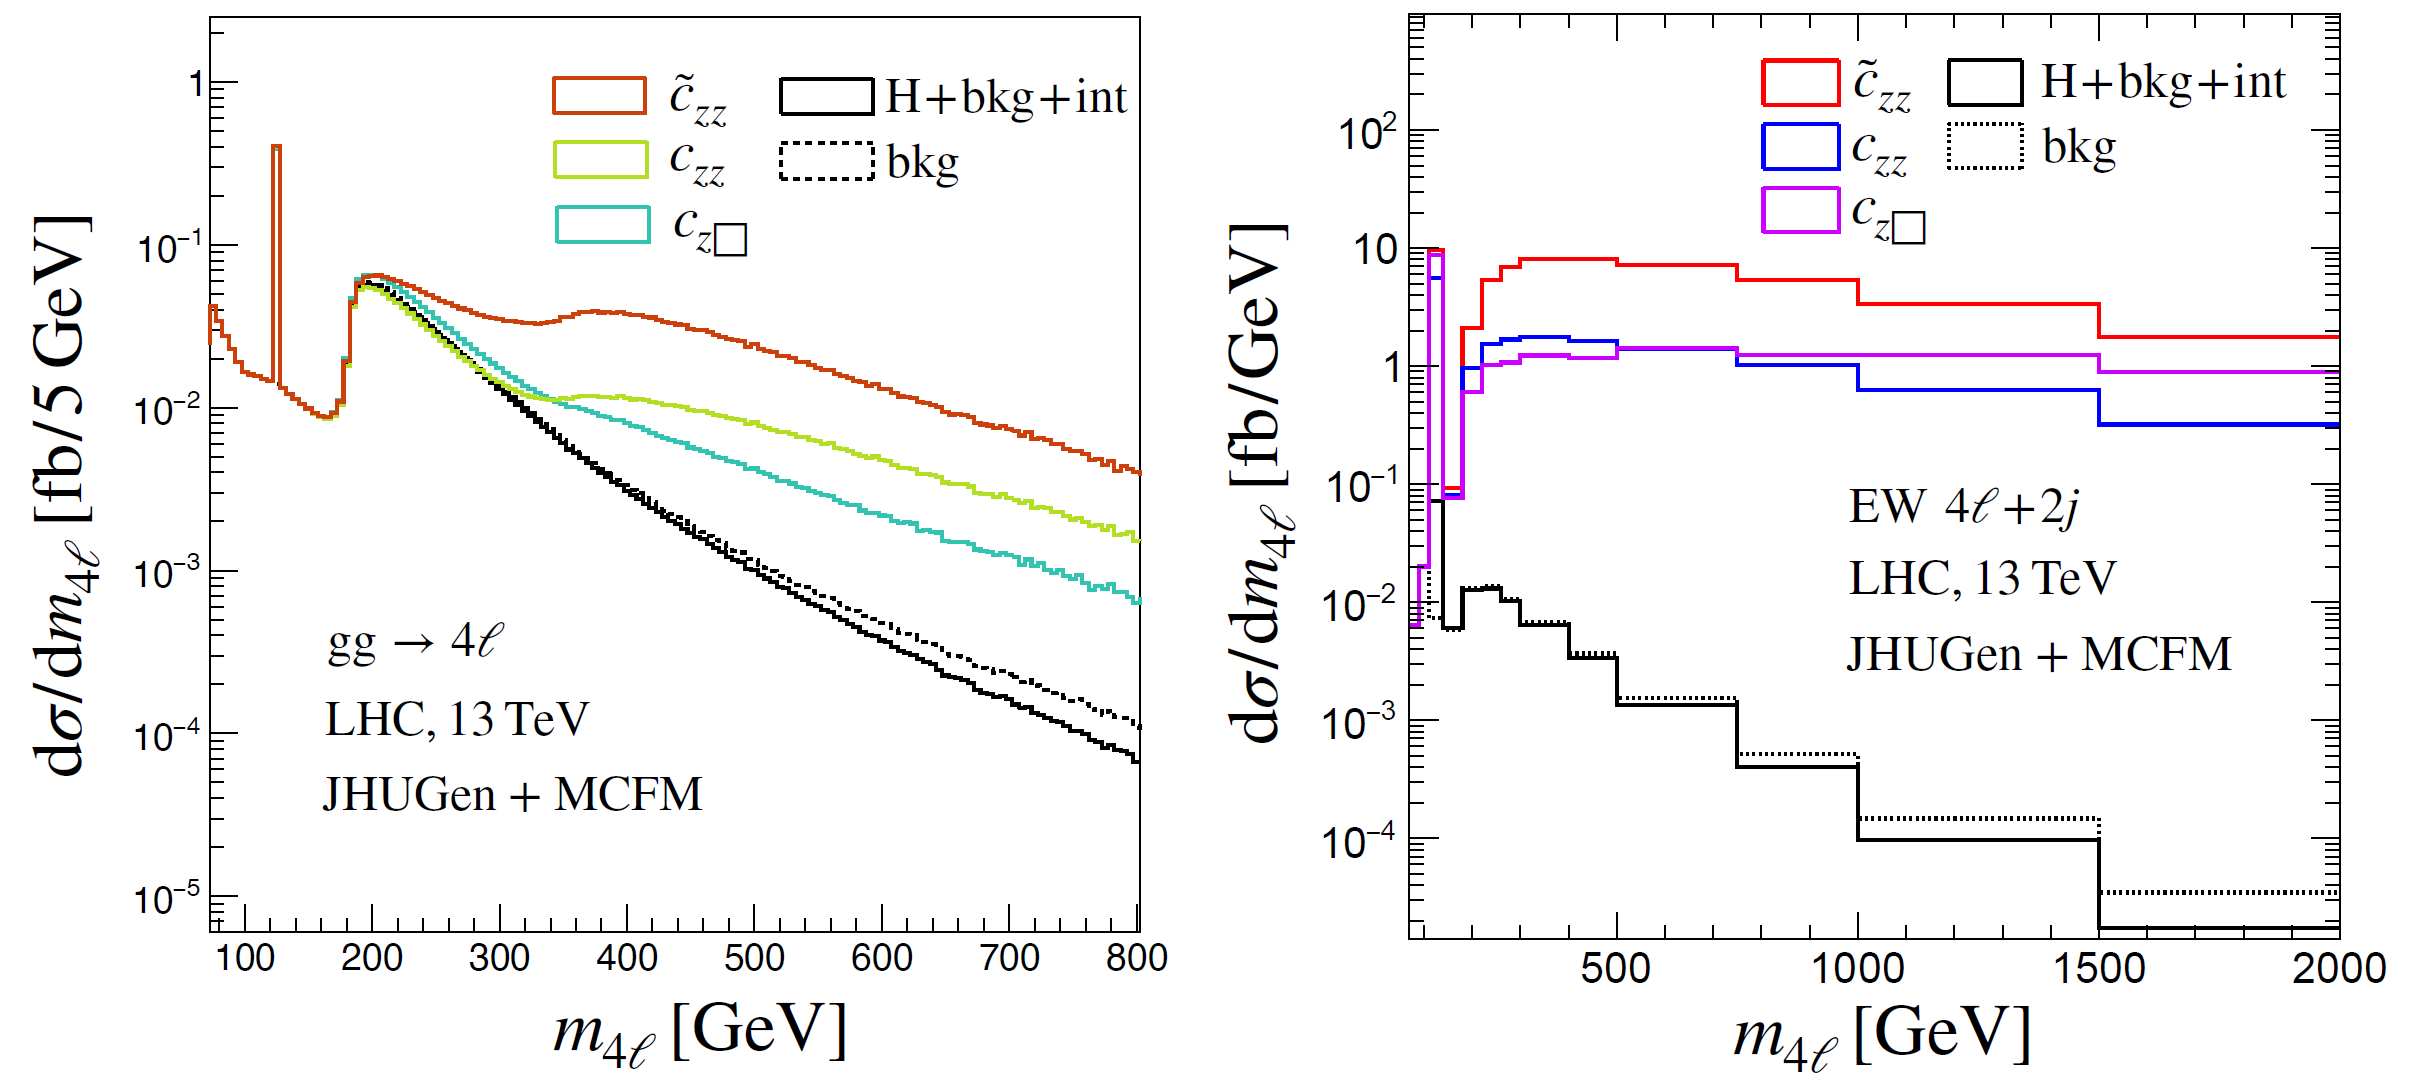
\includegraphics[width=0.8\textwidth,clip] {figures/offshellAC_BSI.png}
\caption{ The four-lepton m4$\ell$ invariant mass distributions for gluon fusion (left) and electroweak production in association with two jets (right) at the LHC with a 13 TeV pp collision energy. The total SM production (“H+bkg+int”) and background-only (“bkg”) components are shown in black. Three operators cz (magenta), czz (blue), and $\tilde{c}$zz (red) are shown
in color, and they are introduced in place of the SM interaction with their strength constrained
to reproduce the SM cross section of the on-shell Higgs boson signal production through gluon
fusion \cite{offshellWGnote}.}
\label{fig:offshellAC_BSI}
\end{figure}

\section{Matrix Element Likelihood Approach}

\begin{figure}
\centering
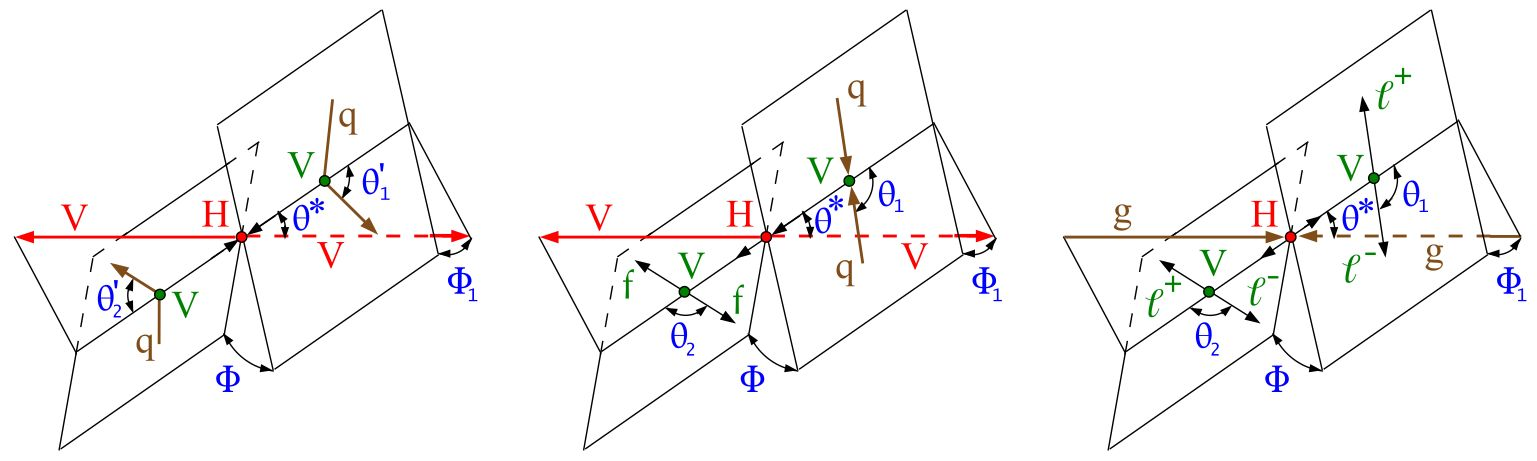
\includegraphics[width=0.8\textwidth,clip] {figures/MELA.jpg}
\caption{}
\label{fig:MELA}
\end{figure}

\begin{equation}
\mathcal{D}_\mathrm{alt}\left(\boldsymbol{\Omega}\right) = \frac{\mathcal{P}_\text{sig}\left(\boldsymbol{\Omega}\right) }
{\mathcal{P}_\text{sig}\left(\boldsymbol{\Omega}\right) +\mathcal{P}_\mathrm{alt}\left(\boldsymbol{\Omega}\right) }
\label{eq:melaD}
\end{equation}


\begin{equation}
\mathcal{D}_\mathrm{int}\left(\boldsymbol{\Omega}\right) =
\frac{\mathcal{P}_\mathrm{int}\left(\boldsymbol{\Omega}\right) }
{2 \ \sqrt{{\mathcal{P}_\text{sig}\left(\boldsymbol{\Omega}\right) \ \mathcal{P}_\mathrm{alt}\left(\boldsymbol{\Omega}\right) }}}
\label{eq:melaDint}
\end{equation}


\begin{figure}
\centering
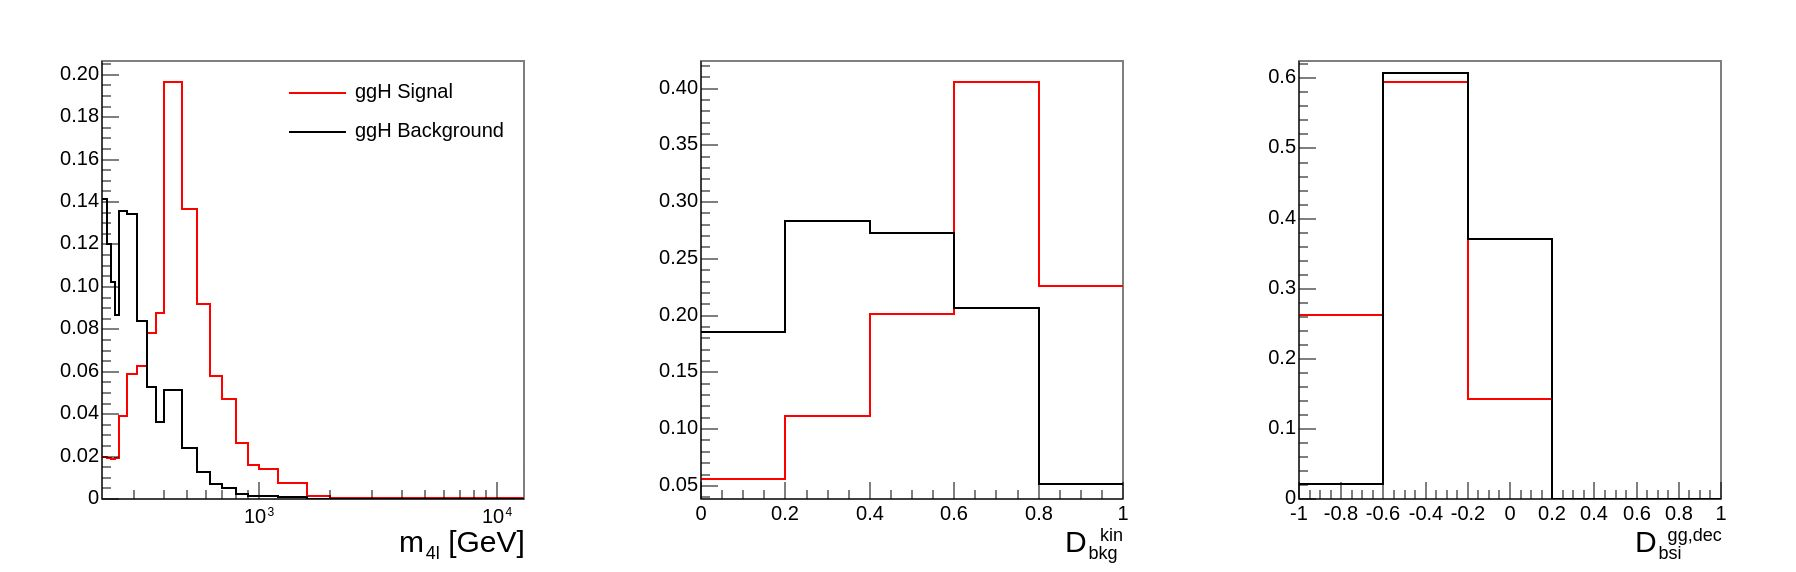
\includegraphics[width=0.8\textwidth,clip] {figures/DiscDists.jpg}
\caption{}
\label{fig:DiscDists}
\end{figure}

In order to perform a dedicated study of a particular kinematic topology, events are split into several mutually 
exclusive categories based on the presence of other particles produced in association with the \Hboson candidate~\cite{Sirunyan:2021rug}.
We use the values of kinematic discriminants and other selection requirements to perform the categorization. 
The definition of these discriminants can be found in Refs.~\cite{Sirunyan:2017exp,Sirunyan:2017tqd,Sirunyan:2019twz,Sirunyan:2021rug}. 
They are calculated using the MELA approach while employing the matrix elements at leading order (LO) in quantum chromodynamics (QCD). 
These discriminants use full kinematic information from the \Hboson and from associated jet production and 
are labeled to indicate a specific topology (2jet) and production mechanism (\VBF, \WH, \ZH), 
which is discriminated against the dominant gluon fusion process:
%$\mathcal{D}_\mathrm{1jet}^{\VBF}$, 
$\mathcal{D}_\mathrm{2jet}^{\VBF}$, 
$\mathcal{D}_\mathrm{2jet}^{\PZ\PH}$,
and $\mathcal{D}_\mathrm{2jet}^{\PW\PH}$. 
%The $\mathcal{D}_\mathrm{2jet}$ discriminants are calculated using both SM and anomalous coupling hypotheses, 
%leading to a set $\mathcal{D}_\mathrm{2jet}^{i}$, all of which 
%are tested in order to maintain high efficiency of \VBF and \VH categorization in the presence of anomalous couplings. 
Calculation of these discriminants is discussed in more detail later with the presented analysis. 

The MELA approach also allows for reweighting between our simulated probability distributions. This has the effect of reducing the number of dedicated 
Monte-Carlo simulations required for this analysis, as well as bolstering the available statistics that can be utilized in our templates for Bayesian analysis. 





Table~\ref{tab:samplesDAStable} provides an accounting of the datasets used.

\begin{table}[h]
	\centering
	\caption{Table of datasets used for Higgs production and $ZZ \rightarrow 4\ell$ decay modes.}
	\label{tab:samplesDAStable}
	\resizebox{\textwidth}{!}{%
		\begin{tabular}{|l|l|}
			\hline
			Process         & Dataset Name      \\ \hline
			$gg \rightarrow H \rightarrow ZZ \rightarrow 4\ell$            & /GluGluToHiggs*ToZZTo*\_M125\_GaSM*\_13TeV\_MCFM701\_pythia8/ \\ 
			$q\bar{q} \rightarrow Hqq \rightarrow ZZqq \rightarrow 4\ell qq$    & /VBFToHiggs0*ToZZTo4l\_M125\_GaSM\_13TeV\_JHUGenV730\_MCFM701\_pythia8/ \\ 
			$q\bar{q} \rightarrow W^{\pm}H \rightarrow ZZZ\rightarrow 4\ell + X$    & /VBFToHiggs0*ToZZTo4l\_M125\_GaSM\_13TeV\_JHUGenV730\_MCFM701\_pythia8/ \\ 
			$q\bar{q} \rightarrow ZH \rightarrow ZZZ \rightarrow 4\ell + X$    & /VBFToHiggs0*ToZZTo4l\_M125\_GaSM\_13TeV\_JHUGenV730\_MCFM701\_pythia8/ \\ \hline
			
			$gg \rightarrow H \rightarrow ZZ \rightarrow 4\ell$            & /GluGluHToZZTo4L\_M*\_13TeV\_powheg2\_JHUGenV7011\_pythia8/ \\ 
			$q\bar{q} \rightarrow Hqq \rightarrow ZZqq \rightarrow 4\ell qq$    & /VBF\_HToZZTo4L\_M*\_13TeV\_powheg2\_JHUGenV7011\_pythia8/ \\
			$q\bar{q} \rightarrow W^{+}H \rightarrow ZZZ\rightarrow 4\ell + X$    &  /WplusH\_HToZZTo4L\_M*\_13TeV\_powheg2-minlo-HWJ\_JHUGenV7011\_pythia8/\\ 
			$q\bar{q} \rightarrow W^{-}H \rightarrow ZZZ\rightarrow 4\ell + X$    &  /WminusH\_HToZZTo4L\_M*\_13TeV\_powheg2-minlo-HWJ\_JHUGenV7011\_pythia8/\\ 
			$q\bar{q} \rightarrow ZH \rightarrow ZZZ \rightarrow 4\ell + X$    & /ZH\_HToZZ\_4LFilter\_M*\_13TeV\_powheg2-minlo-HZJ\_JHUGenV7011\_pythia8/ \\ 
			$t\bar{t} \rightarrow H \rightarrow ZZ \rightarrow 4\ell$    & 	/ttH\_HToZZ\_4LFilter\_M*\_13TeV\_powheg2\_JHUGenV7011\_pythia8/ \\ \hline
			
			$q\bar{q} \rightarrow Hqq \rightarrow ZZqq \rightarrow 4\ell qq$    & /VBFToHiggs0PMContinToZZTo*JJ\_M125\_GaSM\_13TeV\_phantom\_pythia8/ \\ 
			$q\bar{q} \rightarrow Hqq \rightarrow ZZqq \rightarrow 4\ell qq$    & /ZZJJTo4L\_EWK\_TuneCP5\_13TeV-madgraph-pythia8/ \\ \hline
			
			$gg \rightarrow H \rightarrow ZZ \rightarrow 4\ell$            & /Higgs0PMToZZTo4L\_M125\_13TeV\_powheg2\_JHUGenV7011\_pythia8/ \\ 
			$q\bar{q} \rightarrow Hqq \rightarrow ZZqq \rightarrow 4\ell qq$    & /VBFHiggs0PMToZZTo4L\_M125\_13TeV\_JHUGenV7011\_pythia8/ \\ 
			$q\bar{q} \rightarrow W^{\pm}H \rightarrow ZZZ\rightarrow 4\ell + X$    & /WHiggs0PMToZZTo4L\_M125\_13TeV\_JHUGenV7011\_pythia8/ \\ 
			$q\bar{q} \rightarrow ZH \rightarrow ZZZ \rightarrow 4\ell + X$    & /ZHiggs0PMToZZ\_4LFilter\_M125\_13TeV\_JHUGenV7011\_pythia8/ \\ \hline
			
			$qq \rightarrow ZZ \rightarrow 4\ell$                           & /ZZTo4L\_13TeV\_powheg\_pythia8/ \\ \hline
		\end{tabular}%
	}
\end{table}

Here, we have documented inputs used to generate samples that include on-shell events. Most of these samples have already been validated and utilized in analyses such as HIG-18-002, HIG-19-001, HIG-19-009, so we can look to them as a reliable point of comparison for newly generated MC events. There already exist on-shell samples (centered around the 125 GeV Higgs peak) for our dominant production modes generated with POWHEG v2 and JHUGen v7.0.11. We also have as additional samples for electroweak production, on-shell samples generated with JHUGen+JHUGenMELA and off-shell samples of the combined BSI (background+signal+interference) events via Phantom. \\

These samples are valuable in the validation of recently produced off-shell samples for gluon fusion and electroweak production, which were generated using JHUGen v7.3.0 interfaced to MCFM v7.0.1. It is important to note here, as we compare on-shell events between all these samples using the cross-section and branching ratio values from Yellow Report 4, that the off-shell samples share common generator inputs which are not applied to the on-shell samples. These cuts and their associated efficiencies are documented in Table~\ref{tab:geninputtable}.

\begin{table}[h]
	\centering
	\caption{Table of generator-level cuts on jets and leptons.}
	\label{tab:geninputtable}
	\resizebox{\textwidth}{!}{%
		\begin{tabular}{|c|c|c|c|}
			\hline
			Generator           &Sample / Analysis          & Leptons                   & Jets                                \\ \hline
			{JHUGen+MCFM}         &EW off-shell & $pT$ $l_{1,2,3,4} > 3 GeV$, $|\eta$ $l_{1,2,3,4}| < 2.7$ & $pT$ $j_{1,2} >$ 15 GeV, $m_{jj} > $30 GeV, $|\eta$ $j_{1,2}| <$ 6.5, $\Delta R$ $>$ 0.3, $|\Delta\eta$ $j_{1,2}| >$0, $sgn(\eta$ $j_{1}) = \pm sgn(\eta$ $j_{2})$ \\ \cline{2-4} 
			
			&ggH off-shell  & $pT$ $l_{1,2,3,4} > 3 GeV$, $|\eta$ $l_{1,2,3,4}| < 2.7$ & $pT$ $j_{1,2} >$ 15 GeV, $\Delta R$ $>$ 0.4                   \\ \hline
			
			POWHEG+JHUGen                &VBF on-shell  & No specified cuts         & No specified cuts                   \\ \cline{2-4}
			&W$^{-}$H on-shell  & No specified cuts         & No specified cuts                   \\ \cline{2-4}
			&W$^{+}$H on-shell  & No specified cuts         & No specified cuts                   \\ \cline{2-4}
			&ZH on-shell  & No specified cuts         & No specified cuts                   \\ \cline{2-4}
			&ggH on-shell & No specified cuts         & No specified cuts                   \\ \hline
			
			JHUGen+JHUGen           &VBF on-shell         & No specified cuts         & $pT$ $j_{1,2} > 0$ GeV, $\Delta R > 0$ \\ \cline{2-4}
			&WH on-shell         & No specified cuts         & No specified cuts \\ \cline{2-4}
			&ZH on-shell         & No specified cuts         & No specified cuts \\ \hline
			
			Phantom         &EW off-shell (BSI, $4e$) & $pT$ $l_{1,2,3,4} >$ 3 GeV, $|\eta$ $l_{1,2,3,4}| < 2.7$ & $m_{jj} > $30 GeV, $|\eta$ $j_{1,2}| <$ 6.5            \\ \cline{2-4}
			&EW off-shell (BSI, $4\mu$) & $pT$ $l_{1,2,3,4} >$ 3 GeV, $|\eta$ $l_{1,2,3,4}| < 2.7$ & $m_{jj} > $30 GeV, $|\eta$ $j_{1,2}| <$  6.5            \\ \cline{2-4}
			&EW off-shell (BSI, $2e2\mu$) & $pT$ $l_{1,2,3,4} >$ 3 GeV, $|\eta$ $l_{1,2,3,4}| < 2.7$ & $m_{jj} > $30 GeV, $|\eta$ $j_{1,2}| <$ 6.5            \\ \hline
			
		\end{tabular}%
	}
\end{table}



In the \offshell region, the probability density follows Eqs.~(\ref{eq:resonant}) and~(\ref{eq:ponshell}) closely,
with the additional contribution of the interference (``int'') between the signal and background amplitudes,
as well as a cross-feed (``cross'') component discussed below. It is parametrized as 
\ifthenelse{\boolean{true}}{
	\begin{multline}\label{eq:poffshell}
		\mathcal{P}_{jk}(\vec{x};\vec{\xi}_{jk},\vec\zeta) =
		\frac{\mu_j \GH}{\Gref}\mathcal{P}_{jk}^\text{sig} ( \vec{x};\vec{\xi}_{jk})
		+ \sqrt{\frac{\mu_j \GH}{\Gref}}\mathcal{P}_{jk}^\text{int} ( \vec{x};\vec{\xi}_{jk}) \\
		+ \mu_j\mathcal{P}_{jk}^\text{cross} ( \vec{x};\vec{\xi}_{jk})
		+ \mathcal{P}_{jk}^\text{bkg} ( \vec{x};\vec{\xi}_{jk}),
	\end{multline}
}{
	\begin{equation}\label{eq:poffshell}
		\mathcal{P}_{jk}(\vec{x};\vec{\xi}_{jk},\vec\zeta) =
		\frac{\mu_j \GH}{\Gref}\mathcal{P}_{jk}^\text{sig} ( \vec{x};\vec{\xi}_{jk})
		+ \sqrt{\frac{\mu_j \GH}{\Gref}}\mathcal{P}_{jk}^\mathrm{int} ( \vec{x};\vec{\xi}_{jk})
		+ \mu_j\mathcal{P}_{jk}^\text{cross} (\vec{x};\vec{\xi}_{jk})
		+ \mathcal{P}_{jk}^\text{bkg} ( \vec{x};\vec{\xi}_{jk}),
	\end{equation}
}
where $\Gref$ is the reference value of the \Hboson width (not necessarily its SM value)
used in simulation. Otherwise, the definition of the terms is the same as in Eq.~(\ref{eq:ponshell}). 
In the \offshell width analysis, there are two production modes, $j$ (gluon fusion and EW, which includes both \VBF and \VH), 
and three jet-tagged categories, $k$. All lepton flavors and data periods are combined in this analysis.
The contributions from \ttH, \bbH, and \tqH are expected to be negligible in the \offshell region.

The $\mathcal{P}_{jk}^{\text{sig}}$, $\mathcal{P}_{jk}^{\text{int}}$, $\mathcal{P}_{jk}^{\text{cross}}$, and $\mathcal{P}_{jk}^\text{bkg}$ probability densities
are normalized to the expected number of events, and are implemented as binned histograms (templates)
of the observables $\vec{x}$ listed in Table~\ref{tab:categoriesoffshell}.
These templates are obtained as weighted linear combinations of existing simulated signal or background samples.

The \offshell region includes all events with $m_{4\Pell}$ greater than $220\GeV$. 
Other processes can mimic \offshell \Hboson production and decay to four leptons in this region. 
Specifically, we study \onshell signal events in which the \Hboson decays 
to $2\Pell +X$, and $X$ contains further leptons that allow the event to pass the four-lepton selections. 
The dominant \onshell \Hboson process that can contaminate the \offshell region is $\PZ(\Pell\Pell)\PH(2\Pell+X)$, called $\ZH$ cross-feed. 

The $\ZH$ cross-feed contribution is estimated using \onshell 
$\ZH$ samples with $\PH \to \WW$ and $\ZZ$ decays, 
where both hadronic and leptonic decay of the \PZ bosons is allowed. 
The dominant contributions come from the $\PH \to 2\Pell 2\PGn$ and $2\Pell 2\Pq$ final states
produced in association with $\PZ\to 2\Pell$. 
To prevent double counting, \onshell cross-feed events are eliminated from the \offshell simulated samples.

The gluon fusion cross section is calculated using the highest order QCD and EW expansions available 
to simulate inclusive $\PZ\PZ$ production~\cite{deFlorian:2016spz}.
However, event categorization depends on modeling associated jets through \PYTHIA's parton showering and hadronization, 
which involves matching these processes to the hard-scattering production. Off-shell gluon fusion production is generated at LO 
with no associated jets at the matrix element level, and therefore all jets come from \PYTHIA. 
The parton showering and hadronization requires setting the hadronization scale, which can depend on the energy scale 
in the process. In the case of the $\Pg\Pg\to 4\Pell$ process, the energy scale is set at $m_{4\Pell}$.

The EW cross section for the inclusive production of $\PZ\PZ$ and two associated jets is also calculated to the highest order 
QCD and EW expansion available~\cite{deFlorian:2016spz}. 
Contrary to the gluon fusion process, two hard jets, which are typically the leading 
jets in the process, are already generated at the matrix element level in the LO simulation. 
These are the two associated jets in the VBF process, or 
the two jets from the hadronic decay of the associated \PW or \PZ boson. 
Therefore, the dependence on the \PYTHIA parton shower and hadronization 
and its matching to the hard-scattering production is much weaker for these EW processes. 

The categorization efficiency of simulated \ggH and EW \Hboson production can be checked using alternative \POWHEG and \minlo simulations. 
The \POWHEG samples are generated for a wide range of \offshell \Hboson masses at NLO in QCD, 
with one jet generated at the matrix element, and using \PYTHIA matching to simulate additional jets. 
The \minlo simulation of \ggH production is done for \Hboson masses of 125 and $300\GeV$ at NLO in QCD, 
with two jets generated at the matrix element level, and \PYTHIA matching for additional jets.
While the \jhugen categorization efficiencies agree with those using \POWHEG and \minlo 
within the uncertainties of the QCD scale used in \PYTHIA,
for the \ggH process the deviations of the central values and the corresponding uncertainties 
are up to 20\% in the signal-dominated $m_{4\Pell}$ range 300--500\GeV, depending on the category. 
In the EW process, categorization efficiencies from the two approaches typically agree within 5--10\%. 
In all cases, we adjust the categorization efficiency as a function of $m_{4\Pell}$ to match that for the SM signal 
obtained from the \POWHEG samples, and assume the same behavior for 
the background and interference contributions. 
This correction procedure ensures that the total event yield, summed over the three categories,
is unchanged at each value of $m_{4\Pell}$.

Simulation of the $\vec{x}$ observables listed in Table~\ref{tab:categoriesoffshell}
is not affected by the jet modeling in the Untagged category. It is also found that the modeling
of the observables in the jet-tagged categories is nearly the same in the EW process, when 
compared between the direct \MCFM + \jhugen samples and reweighted \POWHEG + \jhugen. 
However, the modeling of jets in the jet-tagged categories for the \ggH process does impact 
the parametrization of the probability distributions. Therefore, within these two jet-tagged categories, 
the gluon fusion process is incorporated through the reweighted \POWHEG + \jhugen simulation. 
This approach allows a more precise matching with the parton shower, thereby 
better describing the associated jet activity. In this case, the samples are reweighted for the appropriate 
model using the \mela package.

\section{Building a $H^{(*)} \rightarrow ZZ^{(*)} \rightarrow 4\ell$ analysis}

\subsection{Selecting and categorizing events}

\subsection{Defining observables}

With up to 13 observables, $\boldsymbol{\Omega}$, describing the \Hboson kinematic distributions in the $2\to 6$ process,
it is a challenging task to perform an optimal analysis in a multidimensional space of observables. 
The \mela approach is designed to reduce the number of observables to the minimum while retaining all essential information. 
Two types of discriminants were defined for either the production or decay process, and we also combine them into a joint 
discriminant for the full $2\to 6$ process where relevant.

These types of discriminants are
\begin{equation}
	\mathcal{D}_\mathrm{alt}\left(\boldsymbol{\Omega}\right) = \frac{\mathcal{P}_\text{sig}\left(\boldsymbol{\Omega}\right) }
	{\mathcal{P}_\text{sig}\left(\boldsymbol{\Omega}\right) +\mathcal{P}_\mathrm{alt}\left(\boldsymbol{\Omega}\right) }
	\label{eq:melaD}
\end{equation}
and
\begin{equation}
	\mathcal{D}_\mathrm{int}\left(\boldsymbol{\Omega}\right) =
	\frac{\mathcal{P}_\mathrm{int}\left(\boldsymbol{\Omega}\right) }
	{2 \ \sqrt{{\mathcal{P}_\text{sig}\left(\boldsymbol{\Omega}\right) \ \mathcal{P}_\mathrm{alt}\left(\boldsymbol{\Omega}\right) }}},
	\label{eq:melaDint}
\end{equation}
where the probability of a certain process $\mathcal{P}$ is calculated using the full kinematics characterized
by $\boldsymbol{\Omega}$ for the processes denoted as ``sig'' for a signal model and ``alt'' for an alternative model,
which could be an alternative \Hboson production mechanism (used to categorize events),
background (to isolate signal), or an alternative \Hboson coupling model (to measure coupling parameters).
The ``int'' label represents the interference between the two model contributions.
The probabilities $\mathcal{P}$ are calculated from the matrix elements provided by the \mela package and
are normalized to give the same integrated cross sections in the relevant phase space of each process.

The selected events are split into three categories: \VBF-tagged, \VH-tagged, and untagged.
A set of discriminants $\mathcal{D}_\text{2jet}$ is constructed, following \Eq{eq:melaD},
where $\mathcal{P}_\text{sig}$ corresponds to the signal probability for the VBF ($\WH$ or $\ZH$)
production hypothesis in the \VBF-tagged (\VH-tagged) category, and $\mathcal{P}_\mathrm{alt}$
corresponds to that of \Hboson production in association with two jets via gluon fusion.
When more than two jets pass the selection criteria, the two jets with the highest $\PT$ are chosen 
for the matrix element calculations. Thereby, the $\mathcal{D}_\text{2jet}$ discriminants separate the 
target production mode of each category from gluon fusion production,
in all cases using only the kinematics of the \Hboson and two associated jets.

The three \offshell categories are summarized in Table~\ref{tab:categoriesoffshell},
and more details were given in Section~\ref{sec:cms}.


\begin{table}[!hbtp]
	\begin{center}
		\caption{
			Summary of the three production categories in the \offshell \mell region. 
			All discriminants are calculated with the \jhugen signal and \MCFM background matrix elements. 
			The \VH interference discriminant in the SM-like analysis hadronic \VH-tagged category is defined as the simple average 
			of the ones corresponding to the \ZH and \WH processes.
		}
		\begin{tabular}{lccc}
			\hline
			\vspace{-0.2cm}  & & & \\
			~~Category              & VBF-tagged & $\V\PH$-tagged  & Untagged \\
			\vspace{-0.2cm}    & & & \\
			\hline
			%
			\vspace{-0.2cm}  & & & \\
			%
			~~Selection
			& ~~$ \mathcal{D}_{\rm 2jet}^{\rm VBF} >0.5$ 
			& ~~$ \mathcal{D}_{\rm 2jet}^{\Z\PH}$ or $ \mathcal{D}_{\rm 2jet}^{\PW\PH}>0.5$
			& ~~Rest of events \\
			%
			&
			& ~~~~
			&   \\
			%
			\vspace{-0.2cm}  & & & \\
			%
			Observables
			&  \mell, $\mathcal{D}^{{\rm VBF}+{\rm dec}}_{\rm bkg}$, $\mathcal{D}_{\rm bsi}^{{\rm VBF}+{\rm dec}}$
			&  \mell, $\mathcal{D}^{\V\PH+{\rm dec}}_{\rm bkg}$, $\mathcal{D}_{\rm bsi}^{\VH+{\rm dec}}$
			&  \mell, $\mathcal{D}^{\rm kin}_{\rm bkg}$, $\mathcal{D}_{\rm bsi}^{{\rm gg},{\rm dec}}$  \\
			& & & \\
			% 
			\hline
			%
		\end{tabular}
		\label{tab:categoriesoffshell}
	\end{center}
\end{table}

In each category of events, three observables $\vec{x}$ are defined following \Eqs{eq:melaD}{eq:melaDint}{and},
as summarized in Table~\ref{tab:categoriesoffshell}, $\vec{x} = \{ \mell, \Dbkg, \Dint \}$.
The \Dbkg observable is calculated differently in the three tagged categories. In the untagged category,
$\mathcal{P}_\text{bkg}$ is calculated for the dominant $\qqbar\to4\ell$ background process.  
The signal and background probabilities include the matrix element probability for a given $\mell$ mass,
as measured in experiment. 
In the \VBF-tagged and \VH-tagged categories, $\mathcal{P}_\text{bkg}$ and $\mathcal{P}_\text{sig}$ include
four-lepton kinematics and kinematic information of the two associated jets.
The $\mathcal{P}_\text{bkg}$ probability density represents the EW and QCD background processes $4\ell+2$\,jets,
while $\mathcal{P}_\text{sig}$ represents EW processes \VBF and \VH. It was found that jet kinematics in the
\Dbkg calculation improves separation of the targeted signal production both against background
and against the \Hboson gluon fusion production.

The third observable, \Dint defined in \Eq{eq:melaDint}, separates the interference
of the SM-like \Hboson coupling and background as an alternative model, and is called
\Dbsi for the signal-background interference in the \offshell region.
In the untagged category, decay information is used in the calculation of \Dint.
In the \VBF-tagged and \VH-tagged categories, production information with the two associated jets is used.

\subsection{Parameterizing the off-shell Higgs boson}

\subsubsection{Cross-feed effect}

\subsection{Parameterizing the on-shell Higgs boson}

\section{Measurement of Higgs boson properties}

\subsection{Off-shell Signal Strength}

\subsection{Higgs boson Width}

\subsection{Kappa Framework}

\subsection{Other measurements}

\subsubsection{Overall Signal Strength}

\subsubsection{Higgs Mass}
